

%% ============================================================
%%  Chapter 2 — Requirements Analysis, Planning and Architecture
%% ============================================================

\chapter{Requirements Analysis, Planning and Architecture}
\minitoc
\newpage

%% ------------------------------------------------------------
\section*{Introduction}
\addcontentsline{toc}{section}{Introduction}
%% ------------------------------------------------------------

This chapter presents the requirements analysis, project planning, and system architecture
of the \textbf{Tesla Academy} platform. It begins by identifying the main actors and their
responsibilities, then describes the functional and non-functional requirements. It
continues with the project planning approach based on Scrum, and concludes with the global
system architecture, the technology stack, and the database design that underpin the
implementation of the platform.

%% ============================================================
\section{Requirements Analysis}
%% ============================================================

Requirements analysis is a fundamental step in any software engineering project. It makes
it possible to clearly define what the system must provide in terms of functionalities and
what quality constraints it must satisfy. In the case of Tesla Academy, this analysis
focuses on the needs of the different user profiles and on the constraints related to
security, performance, scalability, usability, and maintainability.

%% ----------------------------
\subsection{Identification of Actors}
%% ----------------------------

The analysis of the Tesla Academy platform led to the identification of four main actors.
Each actor has specific responsibilities, permissions, and interactions with the system.

\begin{itemize}

  \item \textbf{Super Administrator}: responsible for the global administration of the
        platform. This actor supervises organizations, monitors platform activity, manages
        global indicators, and ensures the proper operation of the system.

  \item \textbf{Organization Administrator}: responsible for the management of a specific
        organization. This actor manages instructors, students, courses, payment settings,
        organization configuration, and the general activity within the organization space.

  \item \textbf{Instructor}: responsible for creating and managing educational content.
        This actor creates courses, organizes lessons and resources, prepares assessments,
        publishes announcements, schedules live sessions, and follows learner progress.

  \item \textbf{Student}: the final user of the platform. This actor accesses courses,
        follows lessons, submits assignments, takes quizzes and tests, joins live sessions,
        interacts with the AI assistant, tracks progress, and obtains certificates when
        success conditions are met.

\end{itemize}

%% ----------------------------
\subsection{Functional Requirements}
%% ----------------------------

Functional requirements describe the main services and actions that the platform must offer
to each actor. In Tesla Academy, these requirements are organized according to the
responsibilities of each user profile.

\subsubsection{Super Administrator Requirements}

The Super Administrator operates at the global platform level and has an overview of all
organizations and system activity.

\begin{itemize}
  \item Manage client organizations by creating, updating, activating, or suspending them;
  \item Consult global platform statistics, including the number of organizations, users,
        courses, and generated revenue;
  \item Monitor the general status of the platform and the services used;
  \item Supervise the global settings required for the proper functioning of the system;
  \item Monitor the general use of AI-related functionalities.
\end{itemize}

\subsubsection{Organization Administrator Requirements}

The Organization Administrator manages the private workspace of an organization. This actor
configures the learning environment, manages users, and supervises educational activities.

\begin{itemize}
  \item Manage instructor and student accounts belonging to the organization;
  \item Create, modify, and organize courses, subjects, chapters, and learning content;
  \item Validate, publish, or reject courses prepared by instructors;
  \item Customize the visual identity and general settings of the organization space;
  \item Consult dashboards to monitor enrollments, learner activity, revenue, and course
        evolution;
  \item Manage categories, prices, course access, and organization-specific parameters;
  \item Configure local payment settings when payment features are enabled;
  \item Configure AI-related settings required for intelligent platform services.
\end{itemize}

\subsubsection{Instructor Requirements}

The Instructor uses the platform to prepare, publish, and monitor educational content.
This role is mainly focused on course creation, assessment preparation, and learner support.

\begin{itemize}
  \item Create and edit courses by defining titles, descriptions, levels, categories, and
        learning objectives;
  \item Structure each course into sections, chapters, and lessons;
  \item Add different types of resources, such as uploaded videos, YouTube videos, PDF
        documents, textual content, and external links;
  \item Prepare quizzes, assignments, and tests using different types of questions;
  \item Review student submissions and consult AI-generated feedback when available;
  \item Schedule and conduct live learning sessions;
  \item Publish announcements for students enrolled in the instructor's courses;
  \item Follow learner progress using dashboards and available statistics;
  \item Generate questions or exercises with the support of AI tools when needed.
\end{itemize}

\subsubsection{Student Requirements}

The Student represents the end user of the platform. This actor accesses learning content,
participates in assessments, and follows progress throughout the learning path.

\begin{itemize}
  \item Browse available courses and enroll in authorized courses;
  \item Purchase paid courses or access free courses;
  \item Watch videos, read PDF documents, and consult resources associated with lessons;
  \item Mark lessons as completed and track course progress;
  \item Take quizzes, tests, and evaluations proposed by instructors;
  \item Submit assignments and consult feedback;
  \item Join live sessions planned by instructors;
  \item Interact with the AI assistant to obtain explanations related to course content;
  \item Consult announcements and take personal notes;
  \item Obtain a certificate after completing a course when the required success conditions
        are met.
\end{itemize}

%% ----------------------------
\subsection{General Use Case Diagram}
%% ----------------------------

\begin{figure}[H]
  \centerline{\includegraphics[width=\textwidth]{use_case_general.png}}
  \caption{General Use Case Diagram of Tesla Academy}
  \label{fig:use_case_general}
\end{figure}

The general use case diagram summarizes the main interactions between the four actors and
the Tesla Academy platform. It highlights the major functionalities related to platform
administration, organization management, course creation, learning activities, assessments,
payments, live sessions, certificates, and AI-powered assistance.

%% ----------------------------
\subsection{Non-Functional Requirements}
%% ----------------------------

Non-functional requirements define the expected qualities of the platform independently of
its specific functionalities. They are essential for ensuring that the system remains
secure, reliable, usable, scalable, and maintainable.

\begin{itemize}

  \item \textbf{Security}: the platform must protect user accounts, organization data,
        educational content, and payment-related information. Each user must access only
        the functionalities authorized by their role.

  \item \textbf{Data confidentiality}: the information of one organization must not be
        accessible to other organizations. Courses, students, payments, and statistics must
        remain isolated within each organization space.

  \item \textbf{Performance}: the main pages of the platform must load quickly in order to
        provide smooth navigation. Access to videos, documents, dashboards, and learning
        activities must remain comfortable as the number of users increases.

  \item \textbf{Availability}: the platform must remain accessible during learning periods,
        payment operations, assessments, and live sessions.

  \item \textbf{Usability}: the interface must be clear and easy to use for different user
        profiles, including administrators, instructors, and students. The main actions
        should be simple to find and perform.

  \item \textbf{Compatibility}: the application must work correctly on modern web browsers
        and adapt to different devices, including computers, tablets, and smartphones.

  \item \textbf{Maintainability}: the solution must be organized in a way that facilitates
        bug fixing, future improvements, and the addition of new features without disrupting
        existing functionalities.

  \item \textbf{Scalability}: the platform must be able to support the growth of the number
        of organizations, users, courses, resources, and AI-related requests.

  \item \textbf{Reliability of AI services}: AI-powered functionalities must provide useful
        and coherent responses while remaining aligned with the educational context of the
        platform.

\end{itemize}

%% ============================================================
\section{Project Planning with Scrum}
%% ============================================================

To organize the development of Tesla Academy, an agile approach based on Scrum was adopted.
This methodology makes it possible to divide the project into short iterations called
sprints, allowing the gradual delivery of the main functionalities of the platform. Scrum
also facilitates adaptation to feedback and improves visibility over the progress of the
project.

%% ----------------------------
\subsection{Definition of Scrum Roles}
%% ----------------------------

\begin{figure}[H]
  \centerline{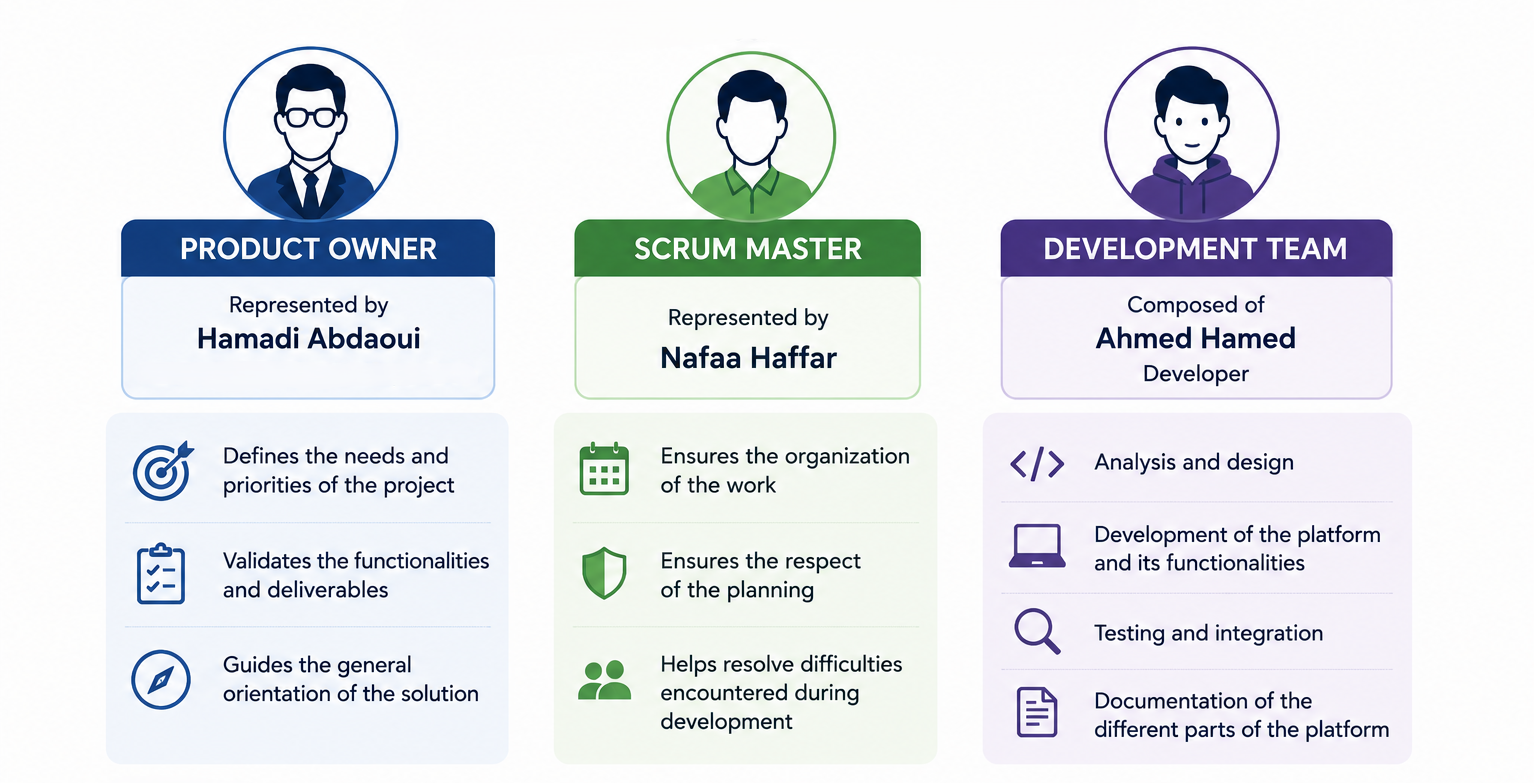
\includegraphics[scale=0.42]{scrum_team_roles.png}}
  \caption{Scrum Team Roles}
  \label{fig:scrum_team_roles}
\end{figure}

Within this project, the Scrum roles are assigned as follows:

\begin{itemize}
  \item \textbf{Product Owner}: represented by the academic and professional supervisors.
        This role contributes to defining the needs, validating the functionalities, and
        guiding the general orientation of the solution;

  \item \textbf{Scrum Master}: represented by the student. This role ensures the
        organization of the work, the respect of the planning, and the resolution of
        difficulties encountered during development;

  \item \textbf{Development Team}: composed of the student, who is responsible for the
        analysis, design, development, testing, integration, and documentation of the
        different parts of the platform.
\end{itemize}

%% ----------------------------
\subsection{Product Backlog}
%% ----------------------------

The Product Backlog contains the main functionalities to be developed in Tesla Academy.
The requirements are expressed as User Stories and organized according to the main actors:
Super Administrator, Organization Administrator, Instructor, Student, and System.

\begingroup
\footnotesize
\setlength{\tabcolsep}{4pt}
\renewcommand{\arraystretch}{1.18}
\begin{longtable}{|p{1.3cm}|p{3cm}|p{2.4cm}|p{7.2cm}|p{1.7cm}|}
  \caption{Product Backlog of Tesla Academy}
  \label{tab:backlog} \\
  \hline
  \textbf{Code} & \textbf{Feature} & \textbf{Actor} & \textbf{User Story} & \textbf{Priority} \\
  \hline
  \endfirsthead

  \hline
  \textbf{Code} & \textbf{Feature} & \textbf{Actor} & \textbf{User Story} & \textbf{Priority} \\
  \hline
  \endhead
  \hline
  \endfoot

  \multicolumn{5}{|l|}\textbf{Sprint 1 -- Authentication and User Management}} \\
  \hline
  US-001 & Registration & Student & Create a student account using an email and password. & Critical \\
  \hline
  US-002 & Login & All & Log in to the platform securely. & Critical \\
  \hline
  US-003 & Logout & All & Log out from the user account. & High \\
  \hline
  US-004 & Forgot password & All & Reset the account password by email. & High \\
  \hline
  US-005 & User profile & All & Update personal information and avatar. & Medium \\
  \hline
  US-006 & Role-based redirection & System & Redirect the user to the appropriate workspace according to their role. & Critical \\
  \hline
  US-007 & Create organization & Super Admin & Create an organization with its main information. & Critical \\
  \hline
  US-008 & Activate / suspend organization & Super Admin & Activate or suspend an organization. & High \\
  \hline
  US-009 & Instructor management & Organization Admin & Add, update, or suspend instructor accounts. & Critical \\
  \hline

  \multicolumn{5}{|l|}\textbf{Sprint 2 -- Organization and Course Management}} \\
  \hline
  US-010 & Create course & Instructor & Create a course with a title, description, level, and category. & Critical \\
  \hline
  US-011 & Edit course & Instructor & Modify the information of an existing course. & High \\
  \hline
  US-012 & Submit course & Instructor & Submit a course to the organization administrator for validation. & Critical \\
  \hline
  US-013 & Validate course & Organization Admin & Approve or reject a course submitted by an instructor. & Critical \\
  \hline
  US-014 & Manage categories & Organization Admin & Create and manage course categories. & High \\
  \hline
  US-015 & Add chapters & Instructor & Organize a course into sections, chapters, and lessons. & Critical \\
  \hline
  US-016 & Add resources & Instructor & Add learning resources such as videos, PDFs, text content, or external links. & Critical \\
  \hline
  US-017 & Upload files & Instructor & Upload videos and documents to the storage service. & Critical \\
  \hline
  US-018 & Archive course & Instructor & Archive a course without permanently deleting it. & Low \\
  \hline

  \multicolumn{5}{|l|}\textbf{Sprint 3 -- Assignments and Learning Experience}} \\
  \hline
  US-019 & Assignment creation & Instructor & Create an assignment by defining its title, instructions, deadline, and evaluation criteria. & Critical \\
  \hline
  US-020 & Assignment resources & Instructor & Attach files, documents, or supporting resources to an assignment. & High \\
  \hline
  US-021 & Assignment publication & Instructor & Publish an assignment and make it available to enrolled students. & High \\
  \hline
  US-022 & Assignment submission & Student & Submit an assignment response with text or attached files before the deadline. & Critical \\
  \hline
  US-023 & Assignment review & Instructor & Review student submissions and provide feedback or grades. & High \\
  \hline
  US-024 & My courses & Student & View the list of courses in which the student is enrolled. & Critical \\
  \hline
  US-025 & Access lesson & Student & Access lesson content such as videos, documents, or text. & Critical \\
  \hline
  US-026 & Complete lesson & Student & Mark a lesson as completed. & Critical \\
  \hline
  US-027 & Progress tracking & Student & Track progress percentage in each course. & High \\
  \hline
  US-028 & Consult assignments & Student & View the list of assignments related to the enrolled courses. & High \\
  \hline
  US-029 & Assignment feedback & Student & Consult feedback or grades received for submitted assignments. & High \\
  \hline
  US-030 & Announcements & Student & Consult announcements published by the instructor. & Medium \\
  \hline

  \multicolumn{5}{|l|}\textbf{Sprint 4 -- Certificates, Dashboards and Course Catalog}} \\
  \hline
  US-031 & Certificate generation & Student & Obtain a certificate after successfully completing a course. & High \\
  \hline
  US-032 & Certificate download & Student & Download the certificate in PDF format. & High \\
  \hline
  US-033 & Student dashboard & Student & View courses, progress, assignments, and certificates. & High \\
  \hline
  US-034 & Instructor dashboard & Instructor & Monitor course statistics, student progress, and assignment submissions. & High \\
  \hline
  US-035 & Publish announcement & Instructor & Publish announcements for enrolled students. & Medium \\
  \hline
  US-036 & Course catalog & Student & View the list of available courses. & Critical \\
  \hline
  US-037 & Course search & Student & Search for a course by keyword. & Critical \\
  \hline
  US-038 & Catalog filters & Student & Filter courses by category, level, or price. & High \\
  \hline
  US-039 & Course details & Student & View detailed information about a course. & Critical \\
  \hline
  US-040 & Reviews and ratings & Student & Rate and comment on a completed course. & Medium \\
  \hline
  US-041 & Free course enrollment & Student & Enroll in a free course without payment. & High \\
  \hline

  \multicolumn{5}{|l|}\textbf{Sprint 5 -- Payments and Live Sessions}} \\
  \hline
  US-042 & Buy course & Student & Purchase a paid course from the platform. & Critical \\
  \hline
  US-043 & Payment confirmation & System & Confirm payment and activate course enrollment. & Critical \\
  \hline
  US-044 & Payment history & Student & Consult payment history. & High \\
  \hline
  US-045 & Schedule live session & Instructor & Schedule a live session with a date, time, and duration. & High \\
  \hline
  US-046 & Start live session & Instructor & Start a live session using the live session service. & High \\
  \hline
  US-047 & Join live session & Student & Join a live session from the student workspace. & High \\
  \hline
  US-048 & Automatic session summary & System & Generate a summary after a live session when transcription data is available. & Medium \\
  \hline

  \multicolumn{5}{|l|}\textbf{Sprint 6 -- AI Features and Deployment}} \\
  \hline
  US-049 & Contextual AI assistant & Student & Ask the intelligent assistant questions related to course content. & Critical \\
  \hline
  US-050 & Assignment feedback with AI & Student & Receive automatic AI-assisted feedback on assignments. & High \\
  \hline
  US-051 & Question generation & Instructor & Generate questions or pedagogical exercises automatically. & High \\
  \hline
  US-052 & AI theme generation & Organization Admin & Generate a visual theme from a textual description. & High \\
  \hline
  US-053 & Theme validation & System & Validate the generated theme before applying it to the platform. & Critical \\
  \hline
  US-054 & Global indicators & Super Admin & Consult global indicators of the platform. & High \\
  \hline
  US-055 & Final validation and deployment & System & Perform final validation, prepare the production environment, and deploy the platform. & Critical \\
  \hline

\end{longtable}
\endgroup

%% ----------------------------
\subsection{User Story Mapping}
%% ----------------------------

\begin{figure}[H]
  \centerline{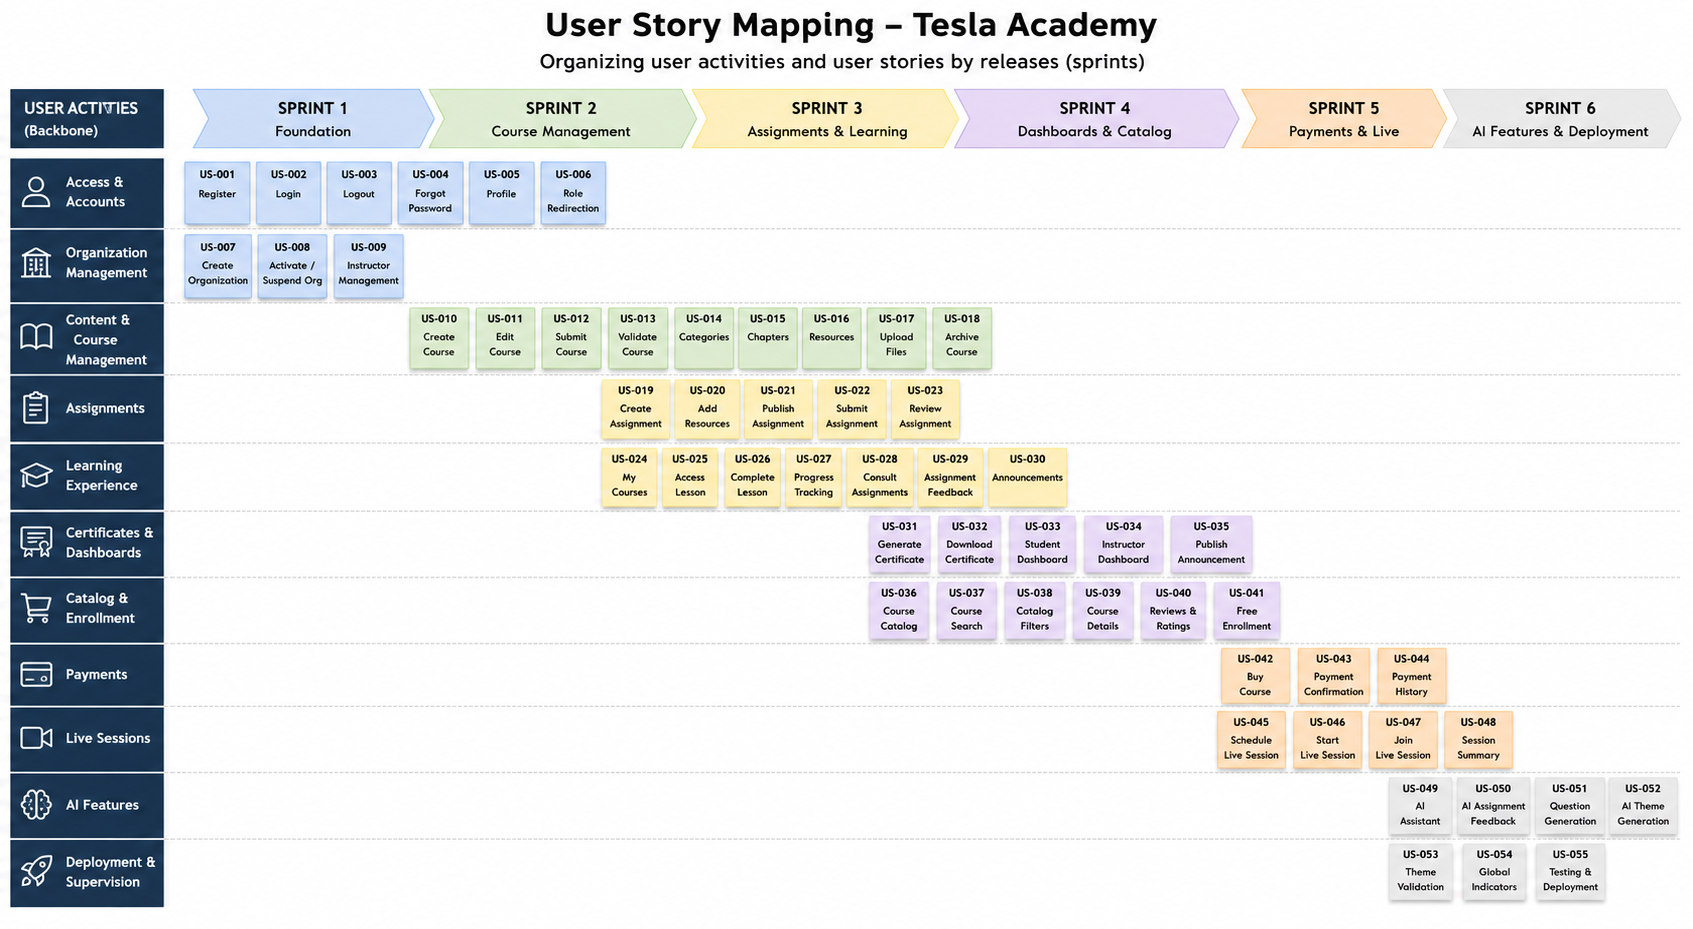
\includegraphics[width=\textwidth]{user_story_mapping.png}}
  \caption{User Story Mapping of Tesla Academy}
  \label{fig:user_story_mapping}
\end{figure}

The User Story Mapping organizes the main functionalities according to user activities and
planned releases. It provides a visual overview of the platform scope and helps prioritize
development according to the value delivered to users.

%% ----------------------------
\subsection{Release and Sprint Planning}
%% ----------------------------

Tesla Academy is planned in \textbf{3 releases} and \textbf{6 sprints}, with each sprint
lasting two weeks. The estimated total duration is therefore \textbf{12 weeks}.

Testing activities are integrated throughout all sprints. Each sprint ends with the
validation of the implemented features. The final sprint is dedicated to AI features,
global validation, deployment preparation, and final adjustments.

\begingroup
\footnotesize
\setlength{\tabcolsep}{4pt}

\begin{longtable}{|p{1.6cm}|p{2.2cm}|p{7.4cm}|p{2.2cm}|}
\caption{Release and Sprint Planning of Tesla Academy}
\label{tab:release_planning} \\
\hline
\textbf{Release} & \textbf{Sprint} & \textbf{Objective} & \textbf{US} \\
\hline
\endfirsthead

\hline
\textbf{Release} & \textbf{Sprint} & \textbf{Objective} & \textbf{US} \\
\hline
\endhead

\hline
\endfoot

\multicolumn{4}{|l|}{\textbf{Release 1 -- Foundation and Core Management}} \\
\hline
R1 & Sprint 1 & Authentication, user profile management, role-based access, organization creation, organization activation, and instructor management. & US-001--009 \\
\hline
R1 & Sprint 2 & Course creation, course editing, course validation, category management, chapter organization, resource management, file upload, and course archiving. & US-010--018 \\
\hline

\multicolumn{4}{|l|}{\textbf{Release 2 -- Learning Experience and Course Access}} \\
\hline
R2 & Sprint 3 & Assignment management, assignment submission, assignment review, lesson access, learner progress tracking, assignment feedback, and announcements. & US-019--030 \\
\hline
R2 & Sprint 4 & Certificate generation, dashboards, course catalog, course search, course filtering, course details, reviews, and free course enrollment. & US-031--041 \\
\hline

\multicolumn{4}{|l|}{\textbf{Release 3 -- Advanced Services and Deployment}} \\
\hline
R3 & Sprint 5 & Paid course purchase, payment confirmation, payment history, live session scheduling, live session start, live session access, and session summary. & US-042--048 \\
\hline
R3 & Sprint 6 & Contextual AI assistant, AI-assisted assignment feedback, question generation, AI theme generation, theme validation, global indicators, final validation, and deployment. & US-049--055 \\
\hline

\multicolumn{3}{|r|}{\textbf{Total -- 6 sprints -- 12 weeks}}
& \textbf{US-001--055} \\
\hline

\end{longtable}
\endgroup

%% ============================================================
%%  GANTT DIAGRAM — To be placed in Chapter 1, Section 1.2.5
%%  After the Release and Sprint Planning table
%%  Add \usepackage{pgfgantt} in your preamble
%% ============================================================

\subsection{Project Gantt Chart}

Figure~\ref{fig:gantt} presents the Gantt chart of the Tesla Academy project,
illustrating the temporal distribution of the six sprints across the twelve-week
development period. Each sprint spans two weeks, and the chart highlights the
sequential progression of releases and the parallel nature of testing activities
integrated throughout the development cycle.

\begin{figure}[H]
\centering
\begin{ganttchart}[
    hgrid,
    vgrid={*{6}{draw=none}, dotted},
    time slot format=isodate,
    time slot unit=day,
    calendar week text={\small W\currentweek},
    title/.style={fill=gray!30, draw=black},
    title label font=\small\bfseries,
    bar/.style={fill=blue!40, draw=blue!60, rounded corners=2pt},
    bar label font=\small,
    group/.style={fill=gray!50, draw=black},
    group label font=\small\bfseries,
    milestone/.style={fill=red!60, draw=red!80, shape=diamond},
    milestone label font=\small,
    link/.style={-latex, thick, draw=gray!70},
    x unit=0.52cm,
    y unit title=0.6cm,
    y unit chart=0.55cm,
    bar height=0.5,
    group height=0.3,
    title height=1,
]{2025-03-03}{2025-05-25}

  %% ---- TITLE ROW (weeks) ----
  \gantttitlecalendar{year, month=shortname, week=1} \\

  %% ---- RELEASE 1 ----
  \ganttgroup{Release 1 — Foundation}{2025-03-03}{2025-03-30} \\
  \ganttbar{Sprint 1 — Auth \& Organization}{2025-03-03}{2025-03-16} \\
  \ganttbar{Sprint 2 — Course Management}{2025-03-17}{2025-03-30} \\
  \ganttbar[bar/.style={fill=green!30, draw=green!60}]
           {Testing R1}{2025-03-24}{2025-03-30} \\

  %% ---- RELEASE 2 ----
  \ganttgroup{Release 2 — Learning Experience}{2025-03-31}{2025-04-27} \\
  \ganttbar{Sprint 3 — Assignments \& Learning}{2025-03-31}{2025-04-13} \\
  \ganttbar{Sprint 4 — Catalog \& Certificates}{2025-04-14}{2025-04-27} \\
  \ganttbar[bar/.style={fill=green!30, draw=green!60}]
           {Testing R2}{2025-04-21}{2025-04-27} \\

  %% ---- RELEASE 3 ----
  \ganttgroup{Release 3 — AI \& Advanced Services}{2025-04-28}{2025-05-25} \\
  \ganttbar{Sprint 5 — Payments \& Live Sessions}{2025-04-28}{2025-05-11} \\
  \ganttbar{Sprint 6 — AI Features \& Deployment}{2025-05-12}{2025-05-25} \\
  \ganttbar[bar/.style={fill=green!30, draw=green!60}]
           {Testing R3}{2025-05-19}{2025-05-25} \\

  %% ---- MILESTONES ----
  \ganttmilestone{R1 Delivery}{2025-03-30} \\
  \ganttmilestone{R2 Delivery}{2025-04-27} \\
  \ganttmilestone{Final Deployment}{2025-05-25} \\

  %% ---- LINKS between sprints ----
  \ganttlink{elem1}{elem2}
  \ganttlink{elem2}{elem5}
  \ganttlink{elem5}{elem6}
  \ganttlink{elem6}{elem9}
  \ganttlink{elem9}{elem10}

\end{ganttchart}
\caption{Project Gantt Chart — Tesla Academy (12 Weeks)}
\label{fig:gantt}
\end{figure}

%% ============================================================
%%  LEGEND (optional, place just below the figure)
%% ============================================================
\begin{center}
\small
\begin{tabular}{cl cl cl}
  \tikz\draw[fill=blue!40, draw=blue!60, rounded corners=2pt] (0,0) rectangle (0.6cm, 0.3cm); & Sprint / Development &
  \tikz\draw[fill=green!30, draw=green!60, rounded corners=2pt] (0,0) rectangle (0.6cm, 0.3cm); & Testing &
  \tikz\draw[fill=red!60, draw=red!80] (0.15cm,0.15cm) -- (0.3cm,0.3cm) -- (0.45cm,0.15cm) -- (0.3cm,0cm) -- cycle; & Milestone \\
\end{tabular}
\end{center}


%% ============================================================
\section{System Architecture and Design}
%% ============================================================

This section presents the overall design of the Tesla Academy platform, describing the
global system architecture, the selected technologies, and the database design that support
its implementation. The architectural choices are driven by the need for multi-tenancy,
security, scalability, maintainability, and seamless integration of AI-powered services.

%% ----------------------------
\subsection{Architecture Overview}
%% ----------------------------

Tesla Academy is designed as a distributed, multi-tier web application. The system is
composed of three main service layers: a \textbf{Next.js frontend}, an \textbf{Express.js
backend API}, and a dedicated \textbf{Python FastAPI AI service}. These layers communicate
through HTTP-based REST interfaces and rely on a shared PostgreSQL database and an
external object storage service.

\begin{figure}[H]
  \centerline{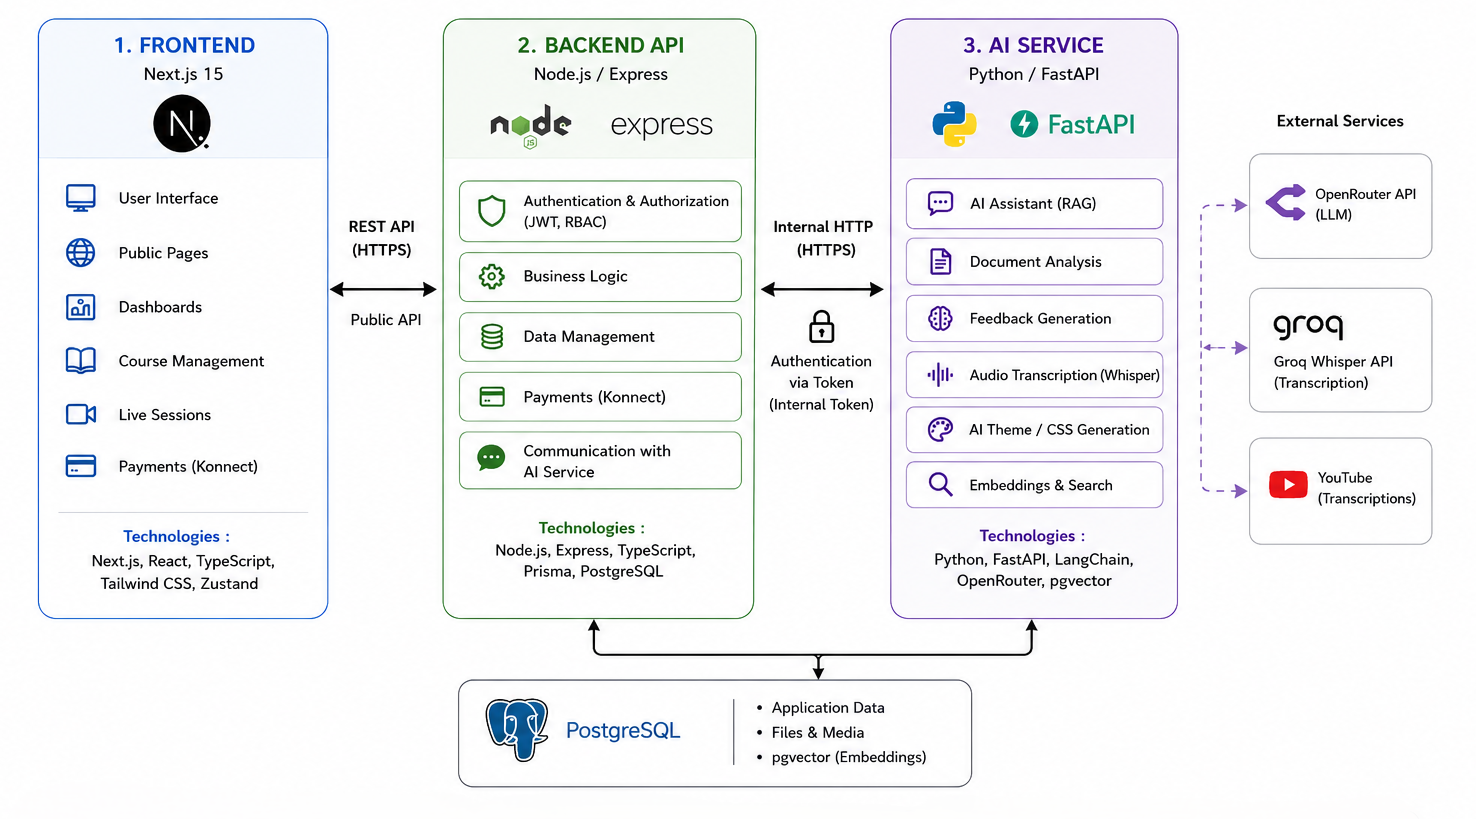
\includegraphics[width=0.85\textwidth]{global_architecture.png}}
  \caption{Global Architecture of Tesla Academy}
  \label{fig:global_architecture}
\end{figure}

%% ----------------------------
\subsection{Multi-Tenancy and Data Isolation}
%% ----------------------------

Tesla Academy is designed around a multi-tenant architecture. Several organizations can use
the same platform and infrastructure while keeping their data, users, courses, settings, and
activities logically isolated. The \texttt{Organization} entity is the root tenant of the
system; most organization-scoped entities carry an \texttt{organizationId} foreign key that
the backend uses to filter data and prevent cross-organization access.

\begin{figure}[H]
  \centerline{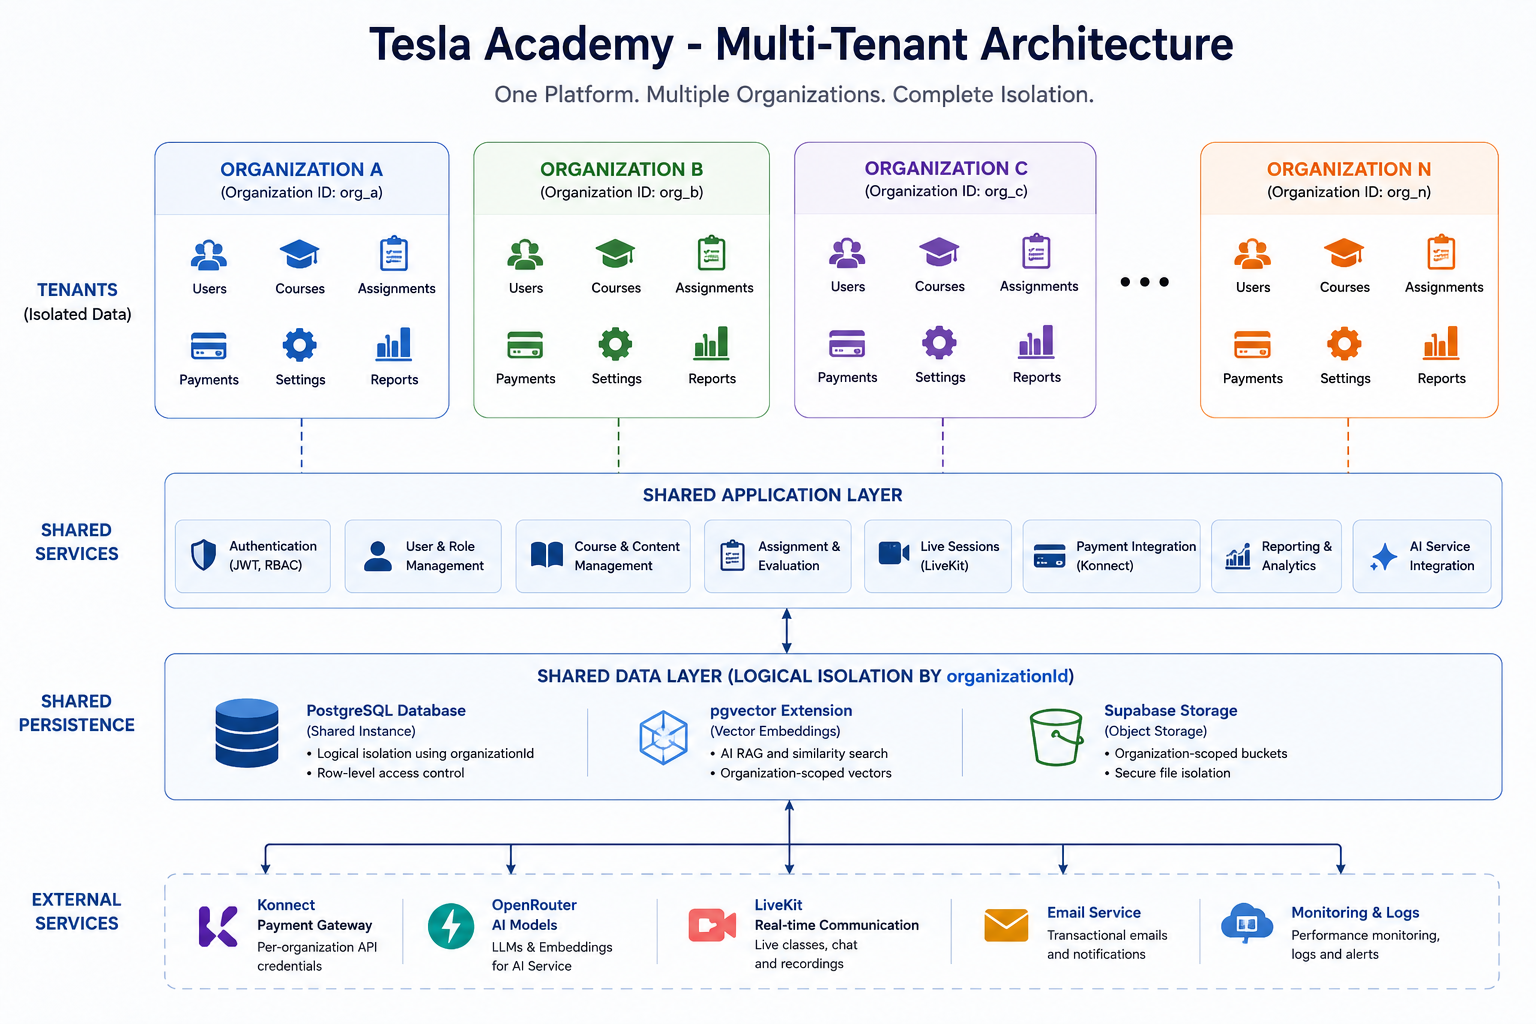
\includegraphics[width=0.75\textwidth]{Multi-Tenant_Architecture.png}}
  \caption{Multi-Tenant Architecture of Tesla Academy}
  \label{fig:Multi-Tenancy}
\end{figure}

This architecture provides data isolation per organization, shared infrastructure for all
tenants, organization-level customization of branding and AI settings, and the ability to
onboard new organizations without deploying separate instances.

%% ----------------------------
\subsection{Technology Stack}
%% ----------------------------

The following tables present the technologies used in each layer of the platform, along
with their respective roles.

\subsubsection{Frontend}

\begingroup
\small
\renewcommand{\arraystretch}{1.4}
\setlength{\tabcolsep}{6pt}
\begin{longtable}{|m{2.8cm}|p{11cm}|}
  \caption{Frontend Technologies}
  \label{tab:frontend_stack} \\
  \hline
  \textbf{Technology} & \textbf{Role and Description} \\
  \hline
  \endfirsthead
  \hline
  \textbf{Technology} & \textbf{Role and Description} \\
  \hline
  \endhead
  \hline
  \endfoot

  
\includegraphics[height=1cm]{nextjs-logo.jpg} &
  \textbf{Next.js / React} --- The frontend is developed with Next.js, a framework built
  on React. It provides routing, page loading optimization, and performance improvements.
  React enables the construction of reusable UI components for the admin, instructor, and
  student spaces. \\
  \hline
  
\includegraphics[height=1cm]{Tailwind_CSS_Logo.svg.png} &
  \textbf{Tailwind CSS / Radix UI / shadcn/ui} --- Tailwind CSS is used to create modern,
  responsive, and consistent interfaces. Radix UI and shadcn/ui provide accessible,
  reusable, and easily customizable components such as menus, forms, dialog boxes, and
  data tables. \\
  \hline
  \raisebox{0.2cm}{\textbf{TanStack}} &
  \textbf{TanStack Query / Zustand / TipTap} --- TanStack Query manages data exchanges
  between the frontend and the backend, facilitating loading, updating, and synchronizing
  displayed information. Zustand manages global application states such as session data and
  user preferences. TipTap serves as a rich text editor for creating and formatting
  educational content. \\
  \hline
  
\includegraphics[height=1cm]{videojs.png} &
  \textbf{Video.js} --- Used on the frontend to ensure smooth playback of video content
  and provide students with a seamless learning experience. \\
  \hline
\end{longtable}
\endgroup

\subsubsection{Backend API}

\begingroup
\small
\renewcommand{\arraystretch}{1.4}
\setlength{\tabcolsep}{6pt}
\begin{longtable}{|m{2.8cm}|p{11cm}|}
  \caption{Backend Technologies}
  \label{tab:backend_stack} \\
  \hline
  \textbf{Technology} & \textbf{Role and Description} \\
  \hline
  \endfirsthead
  \hline
  \textbf{Technology} & \textbf{Role and Description} \\
  \hline
  \endhead
  \hline
  \endfoot

  
\includegraphics[height=1cm]{nodejs_express_logo.png} &
  \textbf{Node.js / Express.js / TypeScript} --- The backend is developed with Node.js and
  Express.js, responsible for processing requests, applying business rules, and
  communicating with the platform's other services. TypeScript improves code quality,
  reduces development errors, and facilitates maintenance. Authentication, role-based
  authorization, data validation, and route protection strengthen API security. \\
  \hline
  
\includegraphics[height=1cm]{postgresql_supabase_logo.png} &
  \textbf{PostgreSQL / Supabase} --- PostgreSQL is used as the relational database
  management system, storing data related to users, courses, assessments, enrollments, and
  organizations. Supabase provides the database infrastructure and additional services,
  notably file storage. \\
  \hline
  
\includegraphics[height=1cm]{prisma_logo.png} &
  \textbf{Prisma ORM} --- Prisma facilitates interactions between the backend and
  PostgreSQL. It enables secure data manipulation, simplifies migration management, and
  produces more readable and maintainable data access code. \\
  \hline
\end{longtable}
\endgroup

\subsubsection{Artificial Intelligence Service}

\begingroup
\small
\renewcommand{\arraystretch}{1.4}
\setlength{\tabcolsep}{6pt}
\begin{longtable}{|m{2.8cm}|p{11cm}|}
  \caption{AI Service Technologies}
  \label{tab:ai_stack} \\
  \hline
  \textbf{Technology} & \textbf{Role and Description} \\
  \hline
  \endfirsthead
  \hline
  \textbf{Technology} & \textbf{Role and Description} \\
  \hline
  \endhead
  \hline
  \endfoot

  
\includegraphics[height=1cm]{astapi_python_logo.png} &
  \textbf{Python / FastAPI} --- The AI service is developed with Python and FastAPI,
  deployed independently of the main backend. Python was chosen for its extensive
  ecosystem of natural language processing libraries; FastAPI enables rapid development
  of high-performance, maintainable APIs. \\
  \hline
  
\includegraphics[height=1cm]{openrouter.png} &
  \textbf{OpenRouter} --- Used as a gateway to access the language models powering the
  platform, notably models from the DeepSeek family. This technology supports the
  intelligent assistant, question generation, automated feedback, and pedagogical
  assistance features. \\
  \hline
  
\includegraphics[height=1cm]{groq_logo.png} &
  \textbf{Groq Whisper / ffmpeg} --- Groq Whisper provides automatic transcription of
  audio and video content. ffmpeg handles media file processing and conversion before
  transcription when necessary. \\
  \hline
  \includegraphics[height=1cm]{pgvector_logo.png} &
  \textbf{pgvector} --- A PostgreSQL extension that enables semantic searches on
  educational resources, enhancing the intelligent assistant's ability to identify the most
  relevant content among available materials. \\
  \hline
\end{longtable}
\endgroup

\subsubsection{External Services}

\begingroup
\small
\renewcommand{\arraystretch}{1.4}
\setlength{\tabcolsep}{6pt}
\begin{longtable}{|m{2.8cm}|p{11cm}|}
  \caption{External Services}
  \label{tab:external_services} \\
  \hline
  \textbf{Technology} & \textbf{Role and Description} \\
  \hline
  \endfirsthead
  \hline
  \textbf{Technology} & \textbf{Role and Description} \\
  \hline
  \endhead
  \hline
  \endfoot

  
\includegraphics[height=1cm]{livekit_logo.png} &
  \textbf{LiveKit} --- Manages live training sessions by providing real-time audio and
  video communication between instructors and students, supporting synchronous interactions
  that complement the available educational resources. \\
  \hline
  
\includegraphics[height=1cm]{konnect_logo.png} &
  \textbf{Konnect} --- The payment gateway integrated into Tesla Academy, enabling users
  to make secure payments for course purchases and ensuring complete management of the
  payment process up to transaction validation. \\
  \hline
  
\includegraphics[height=1cm]{supabaselogo.png} &
  \textbf{Supabase Storage} --- Used for storing educational resources including videos,
  documents, and uploaded files, providing centralized and secure management of educational
  content. \\
  \hline
\end{longtable}
\endgroup

%% ----------------------------
\subsection{Development Tools}
%% ----------------------------

\begingroup
\small
\renewcommand{\arraystretch}{1.25}
\setlength{\tabcolsep}{4pt}
\begin{longtable}{|p{4cm}|p{3.5cm}|p{7cm}|}
\caption{Development Tools Used}
\label{tab:dev_tools} \\
\hline
\textbf{Category} & \textbf{Tool} & \textbf{Usage} \\
\hline
\endfirsthead
\hline
\textbf{Category} & \textbf{Tool} & \textbf{Usage} \\
\hline
\endhead
\hline
\endfoot
Development Environment & Visual Studio Code & Development of frontend, backend and AI service \\
\hline
Version Control & Git / GitHub & Source code management and version tracking \\
\hline
API Testing & Insomnia & Testing routes and API requests \\
\hline
Database & Prisma Studio & Data browsing and verification \\
\hline
Design & Figma & Creation of user interface mockups \\
\hline
Diagrams & draw.io & Creation of UML and architecture diagrams \\
\hline
Project Management & Notion & Task management and project tracking \\
\hline
\end{longtable}
\endgroup

%% ----------------------------
\subsection{Database Design}
%% ----------------------------

The data model of Tesla Academy is implemented as a relational schema in PostgreSQL and
managed through Prisma ORM. The schema is designed to support multi-tenancy through the
systematic use of \texttt{organizationId} foreign keys on organization-scoped entities.

\begin{figure}[H]
  \centerline{\includegraphics[width=\textwidth]{erd.png}}
  \caption{Entity Relationship Diagram of Tesla Academy}
  \label{fig:erd}
\end{figure}

The platform's data model is organized around the following principal entities:

\begin{itemize}

  \item \textbf{Organization and OrganizationConfig}: the root tenant entity, storing
        identification details such as name, slug, subdomain, and activation status, along
        with a configuration record that holds branding, payment parameters, AI provider
        settings, and feature flags for each organization.

  \item \textbf{User and Teacher}: users belong to an organization and carry a role
        (administrator, teacher, or student). The Teacher entity extends the user record
        with instructor-specific data linked to courses, assignments, and schedules.

  \item \textbf{Batch (Course) and Content Hierarchy}: a Batch represents a training
        course. Course content is organized hierarchically into Subjects, Chapters, Topics,
        and Content records (videos, PDFs, text blocks, or external links), allowing
        instructors to structure material into clear learning units.

  \item \textbf{Assignment and AssignmentSubmission}: an Assignment stores the title,
        instructions, deadline, and maximum mark. Each student response is recorded in an
        AssignmentSubmission, which holds the submitted text, attached files, status,
        grade, and optional AI-generated feedback.

  \item \textbf{BatchEnrollment and BatchCertificateIssue}: BatchEnrollment tracks which
        students are enrolled in which courses. BatchCertificateIssue records certificates
        awarded to students upon successful course completion, with a unique credential
        identifier and issue date.

  \item \textbf{Order}: records purchase transactions, storing buyer identity, purchased
        entity, amount, currency, payment provider reference, and payment status.

  \item \textbf{Schedule}: represents a scheduled live session, storing the title,
        date, duration, associated course, LiveKit room information, and optional
        transcription data used for post-session summarization.

  \item \textbf{Report}: stores generated analytics used by administrators to monitor
        platform activity, learning progress, payments, and AI-related usage.

\end{itemize}

%% ------------------------------------------------------------
\section*{Conclusion}
\addcontentsline{toc}{section}{Conclusion}
%% ------------------------------------------------------------

This chapter presented the requirements analysis, project planning, and system architecture
of Tesla Academy. It identified the main actors and their responsibilities, described the
functional and non-functional requirements, and introduced the general use case diagram.
The Scrum-based planning defined the Product Backlog, User Story Mapping, and a release
plan organized into three releases and six two-week sprints.

The chapter also described the global multi-service architecture, the technology stack
chosen to maximize productivity, type safety, and maintainability, and the relational
database design that supports the platform's multi-tenant and AI-powered requirements.
The next chapter focuses on the implementation of Release 1, covering authentication,
user management, organization management, and course structure functionalities.